\documentclass{beamer}

\pdfmapfile{+sansmathaccent.map}


\mode<presentation>
{
	\usetheme{Warsaw} % or try Darmstadt, Madrid, Warsaw, Rochester, CambridgeUS, ...
	\usecolortheme{seahorse} % or try seahorse, beaver, crane, wolverine, ...
	\usefonttheme{serif}  % or try serif, structurebold, ...
	\setbeamertemplate{navigation symbols}{}
	\setbeamertemplate{caption}[numbered]
} 


%%%%%%%%%%%%%%%%%%%%%%%%%%%%
% itemize settings


%%%%%%%%%%%%%%%%%%%%%%%%%%%%
% itemize settings

\definecolor{myhotpink}{RGB}{255, 80, 200}
\definecolor{mywarmpink}{RGB}{255, 60, 160}
\definecolor{mylightpink}{RGB}{255, 80, 200}
\definecolor{mypink}{RGB}{255, 30, 80}
\definecolor{mydarkpink}{RGB}{155, 25, 60}

\definecolor{mypaleblue}{RGB}{240, 240, 255}
\definecolor{mylightblue}{RGB}{120, 150, 255}
\definecolor{myblue}{RGB}{90, 90, 255}
\definecolor{mygblue}{RGB}{70, 110, 240}
\definecolor{mydarkblue}{RGB}{0, 0, 180}
\definecolor{myblackblue}{RGB}{40, 40, 120}

\definecolor{myblackturquoise}{RGB}{5, 53, 60}
\definecolor{mydarkdarkturquoise}{RGB}{8, 93, 110}
\definecolor{mydarkturquoise}{RGB}{28, 143, 150}
\definecolor{mypaleturquoise}{RGB}{230, 255, 255}
\definecolor{myturquoise}{RGB}{48, 213, 200}

\definecolor{mygreen}{RGB}{0, 200, 0}
\definecolor{mydarkgreen}{RGB}{0, 120, 0}
\definecolor{mygreen2}{RGB}{245, 255, 230}

\definecolor{mygrey}{RGB}{120, 120, 120}
\definecolor{mypalegrey}{RGB}{160, 160, 160}
\definecolor{mydarkgrey}{RGB}{80, 80, 160}

\definecolor{mydarkred}{RGB}{160, 30, 30}
\definecolor{mylightred}{RGB}{255, 150, 150}
\definecolor{myred}{RGB}{200, 110, 110}
\definecolor{myblackred}{RGB}{120, 40, 40}

\definecolor{mygreen}{RGB}{0, 200, 0}
\definecolor{mygreen2}{RGB}{205, 255, 200}

\definecolor{mydarkcolor}{RGB}{60, 25, 155}
\definecolor{mylightcolor}{RGB}{130, 180, 250}

\setbeamertemplate{itemize items}[default]

\setbeamertemplate{itemize item}{\color{myblackturquoise}$\blacksquare$}
\setbeamertemplate{itemize subitem}{\color{mydarkdarkturquoise}$\blacktriangleright$}
\setbeamertemplate{itemize subsubitem}{\color{mygray}$\blacksquare$}

\setbeamercolor{palette quaternary}{fg=white,bg=myblackturquoise}
\setbeamercolor{titlelike}{parent=palette quaternary}

\setbeamercolor{palette quaternary2}{fg=black,bg=mypaleblue}
\setbeamercolor{frametitle}{parent=palette quaternary2}

\setbeamerfont{frametitle}{size=\Large,series=\scshape}
\setbeamerfont{framesubtitle}{size=\normalsize,series=\upshape}





%%%%%%%%%%%%%%%%%%%%%%%%%%%%
% block settings

\setbeamercolor{block title}{bg=red!30,fg=black}

\setbeamercolor*{block title example}{bg=mygreen!40!white,fg=black}

\setbeamercolor*{block body example}{fg= black, bg= mygreen2}


%%%%%%%%%%%%%%%%%%%%%%%%%%%%
% URL settings
\hypersetup{
	colorlinks=true,
	linkcolor=blue,
	filecolor=blue,      
	urlcolor=blue,
}

%%%%%%%%%%%%%%%%%%%%%%%%%%

\renewcommand{\familydefault}{\rmdefault}

\usepackage{amsmath}
\usepackage{mathtools}

\usepackage{subcaption}

\usepackage{qrcode}

\DeclareMathOperator*{\argmin}{arg\,min}
\newcommand{\bo}[1] {\mathbf{#1}}

\newcommand{\R}{\mathbb{R}} 
\newcommand{\T}{^\top}     



\newcommand{\mydate}{Fall 2023}

\newcommand{\mygit}{\textcolor{blue}{\href{https://github.com/SergeiSa/Control-Theory-Slides-Spring-2023}{github.com/SergeiSa/Control-Theory-Slides-Spring-2023}}}

\newcommand{\myqr}{ \textcolor{black}{\qrcode[height=1.5in]{https://github.com/SergeiSa/Control-Theory-Slides-Spring-2023}}
}

\newcommand{\myqrframe}{
	\begin{frame}
		\centerline{Lecture slides are available via Github, links are on Moodle}
		\bigskip
		\centerline{You can help improve these slides at:}
		\centerline{\mygit}
		\bigskip
		\myqr
	\end{frame}
}


\newcommand{\bref}[2] {\textcolor{blue}{\href{#1}{#2}}}

%%%%%%%%%%%%%%%%%%%%%%%%%%%%
% code settings

\usepackage{listings}
\usepackage{color}
% \definecolor{mygreen}{rgb}{0,0.6,0}
% \definecolor{mygray}{rgb}{0.5,0.5,0.5}
\definecolor{mymauve}{rgb}{0.58,0,0.82}
\lstset{ 
	backgroundcolor=\color{white},   % choose the background color; you must add \usepackage{color} or \usepackage{xcolor}; should come as last argument
	basicstyle=\footnotesize,        % the size of the fonts that are used for the code
	breakatwhitespace=false,         % sets if automatic breaks should only happen at whitespace
	breaklines=true,                 % sets automatic line breaking
	captionpos=b,                    % sets the caption-position to bottom
	commentstyle=\color{mygreen},    % comment style
	deletekeywords={...},            % if you want to delete keywords from the given language
	escapeinside={\%*}{*)},          % if you want to add LaTeX within your code
	extendedchars=true,              % lets you use non-ASCII characters; for 8-bits encodings only, does not work with UTF-8
	firstnumber=0000,                % start line enumeration with line 0000
	frame=single,	                   % adds a frame around the code
	keepspaces=true,                 % keeps spaces in text, useful for keeping indentation of code (possibly needs columns=flexible)
	keywordstyle=\color{blue},       % keyword style
	language=Octave,                 % the language of the code
	morekeywords={*,...},            % if you want to add more keywords to the set
	numbers=left,                    % where to put the line-numbers; possible values are (none, left, right)
	numbersep=5pt,                   % how far the line-numbers are from the code
	numberstyle=\tiny\color{mygray}, % the style that is used for the line-numbers
	rulecolor=\color{black},         % if not set, the frame-color may be changed on line-breaks within not-black text (e.g. comments (green here))
	showspaces=false,                % show spaces everywhere adding particular underscores; it overrides 'showstringspaces'
	showstringspaces=false,          % underline spaces within strings only
	showtabs=false,                  % show tabs within strings adding particular underscores
	stepnumber=2,                    % the step between two line-numbers. If it's 1, each line will be numbered
	stringstyle=\color{mymauve},     % string literal style
	tabsize=2,	                   % sets default tabsize to 2 spaces
	title=\lstname                   % show the filename of files included with \lstinputlisting; also try caption instead of title
}


%%%%%%%%%%%%%%%%%%%%%%%%%%%%
% URL settings
\hypersetup{
	colorlinks=false,
	linkcolor=blue,
	filecolor=blue,      
	urlcolor=blue,
}

%%%%%%%%%%%%%%%%%%%%%%%%%%

%%%%%%%%%%%%%%%%%%%%%%%%%%%%
% tikz settings

\usepackage{tikz}
\tikzset{every picture/.style={line width=0.75pt}}


\title{Gearbox, Nonlinearity}
\subtitle{Mechatronics, Lecture 8}
\author{by Sergei Savin}
\centering
\date{\mydate}



\begin{document}
\maketitle



\begin{frame}{Content}
\begin{itemize}
\item Gear systems
\begin{itemize}
	\item Cylindrical gears
	\item Worm gears
	\item Planetary gears
	\item Strain wave gears
\end{itemize}
\item Dry friction
\item Stiction
\item Backlash
\end{itemize}
\end{frame}




\begin{frame}{Gear systems}
	% \framesubtitle{O}
	\begin{flushleft}
		
		Motors often require a gear system (gearing, gearbox, transmission, reducers) to lower the output shaft speed and increase the output torque.
		
		\bigskip
		
		
		There is a great variety of possible gear systems, however, a few are especially popular. They differ from each other in terms of \emph{reduction ratio}, \emph{backdrivability}, mechanical complexity and other characteristics.
		
	\end{flushleft}
\end{frame}



\begin{frame}{Cylindrical gears}
	% \framesubtitle{O}
	\begin{flushleft}
		
		% TODO: \usepackage{graphicx} required
		\begin{figure}
			\centering
			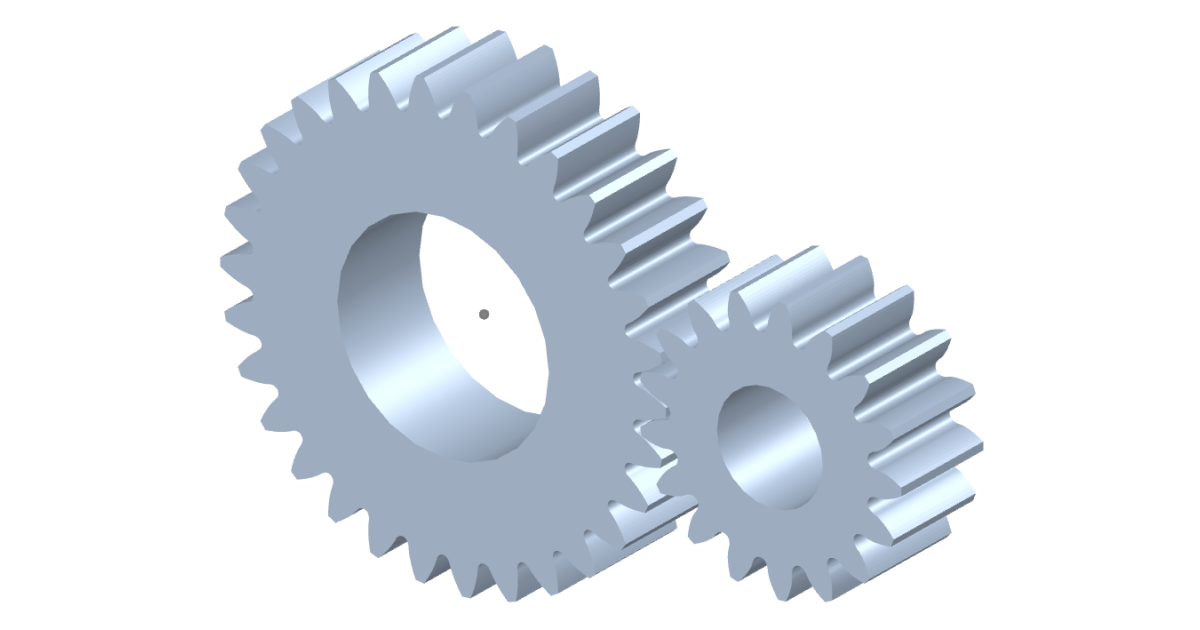
\includegraphics[width=0.7\linewidth]{cylindrical}
			\caption{Cylindrical gears}
			\label{fig:cylindrical}
		\end{figure}
		
		Cylindrical gears usually have low or medium reduction ratio. When reduction ratio is low, they are backdrivable. 
		
	\end{flushleft}
\end{frame}

\begin{frame}{Worm gears}
	% \framesubtitle{O}
	\begin{flushleft}
		
% TODO: \usepackage{graphicx} required
\begin{figure}
	\centering
	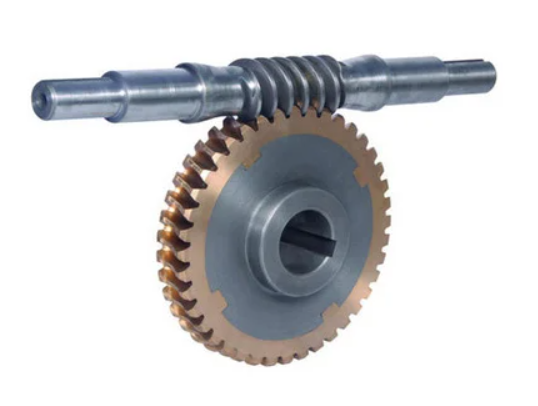
\includegraphics[width=0.7\linewidth]{worm}
	\caption{Worm gear}
	\label{fig:worm}
\end{figure}

		
		Worm gears usually have medium or high reduction ratio. Not backdrivable.
		
	\end{flushleft}
\end{frame}


\begin{frame}{Planetary gears}
	% \framesubtitle{O}
	\begin{flushleft}
		
		% TODO: \usepackage{graphicx} required
		\begin{figure}
			\centering
			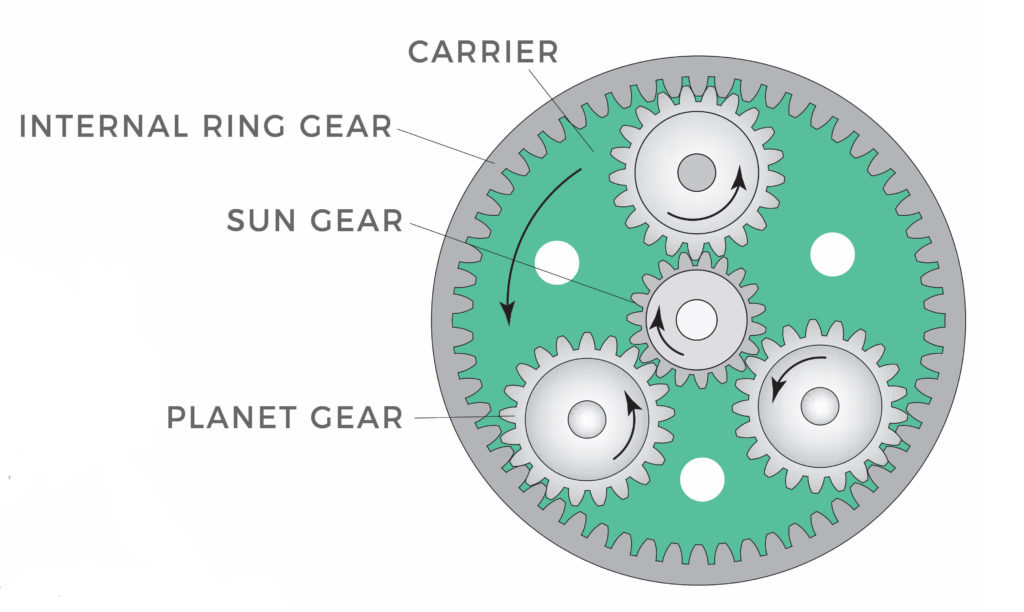
\includegraphics[width=0.7\linewidth]{Planetary}
			\caption{Planetary gear.  \bref{https://www.linearmotiontips.com/why-are-planetary-gearboxes-preferred-for-servo-applications/}{Image credit.} }
			\label{fig:worm}
		\end{figure}
		
		Planetary gears usually have medium or high reduction ratio. Usually are not backdrivable.
		
		
	\end{flushleft}
\end{frame}


\begin{frame}{Strain wave gears}
	% \framesubtitle{O}
	\begin{flushleft}
		
		% TODO: \usepackage{graphicx} required
		\begin{figure}
			\centering
			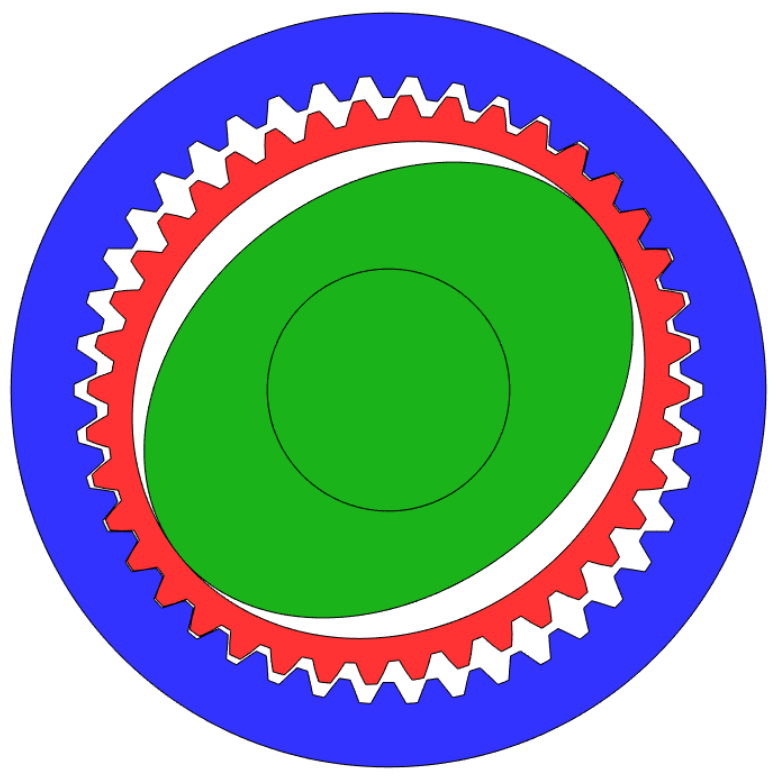
\includegraphics[width=0.5\linewidth]{strain_wave}
			\caption{Strain wave gear. }
			\label{fig:worm}
		\end{figure}
		
		Strain wave gears usually have high reduction ratio. Not backdrivable.
		
		
	\end{flushleft}
\end{frame}



\begin{frame}{Non-linearity in gear systems}
	% \framesubtitle{O}
	\begin{flushleft}
		
		There are typical sources of non-linearity in gear systems: 
		
		\begin{itemize}
			\item Dry friction, causing "dead zone" effect - zero output shaft angular velocity with non-zero input voltage.
			
			\item Backlash, causing, e.g. non-zero output shaft angular velocity with zero input voltage.
		\end{itemize}  
		
		
	\end{flushleft}
\end{frame}




\begin{frame}{Dry friction, 1}
	% \framesubtitle{O}
	\begin{flushleft}
		
		Dry friction can be described like this:
		
		\begin{itemize}
			\item When there is no motion, dry friction prevents the motion from starting as long as the force needed to accomplish it is less than maximum friction force.
			
			\item When there is motion, dry friction force is equal it its maximum value.
		\end{itemize}  
		
		This is one of many possible dry friction models.		
		
	\end{flushleft}
\end{frame}


\begin{frame}{Dry friction, 2}
	% \framesubtitle{O}
	\begin{flushleft}
		
		Let $\omega$ describe angular velocity of the output shaft, and $\tau_{f, \text{max}}$ be the maximum value of the dry friction torque. Assuming that $\omega 
		\geq 0$ the dry friction model can be described:
		
		\begin{equation}
			\begin{cases}
				J \frac{d \omega}{dt} + F \omega = C_\tau I - \tau_f,  \\
				(\tau_f -  \tau_{f, \text{max}}) \omega = 0, \\
				\tau_f \leq \tau_{f, \text{max}}
			\end{cases}
		\end{equation}
		
		The constraint $(\tau_f -  \tau_{f, \text{max}}) \omega = 0$ is a complementarity constraint. For it to hold, either $\tau_f = \tau_{f, \text{max}}$ should hold, or the velocity should be zero $\omega = 0$.
		
	\end{flushleft}
\end{frame}


\begin{frame}{Dry friction, 3}
	% \framesubtitle{O}
	\begin{flushleft}
		
		We have two basic scenarios:
		
		\begin{enumerate}
			\item $\omega = 0$ and $\tau_f \leq \tau_{f, \text{max}}$, giving us $C_\tau I - \tau_f = 0$.
			
			\item $\omega \neq 0$ and $\tau_f = \tau_{f, \text{max}}$, giving us $J \frac{d \omega}{dt} + F \omega = C_\tau I - \tau_{f, \text{max}}$.
		\end{enumerate}
		
		For the switch from the first scenario to the second one to occur, the friction force has to reach $\tau_{f, \text{max}}$, allowing positive acceleration.
		
		\bigskip
		
		For the switch from the second scenario to the first one to occur, velocity has to reach zero and the friction force should be less than or equal to the maximum value.
		
	\end{flushleft}
\end{frame}



\begin{frame}{Dry friction, 4}
	% \framesubtitle{O}
	\begin{flushleft}
		
		During the first scenario, $C_\tau I = \tau_f$. For the motion to start (for the transition to the second scenario to occur) $\tau_f$ should reach the value $\tau_{f, \text{max}}$, meaning we could find the value of the current during the transition $I_{tr}$:
		
		\begin{equation}
			C_\tau I_{tr} = \tau_{f, \text{max}}
		\end{equation}
		
		This implies $I_{tr} = \frac{\tau_{f, \text{max}}}{C_\tau}$.  Let us consider a steady-state solution of the electrical equation that leads to the output of such current:
		%
		\begin{align}
			R I_{tr} = u_{tr}
		\end{align}
		
		where $u_{tr} = \frac{R}{C_\tau} \tau_{f, \text{max}}$ is a transition voltage.
		
	\end{flushleft}
\end{frame}



\begin{frame}{Dry friction - stiction, 1}
	% \framesubtitle{O}
	\begin{flushleft}
		
		Stiction model of dry friction can be described like this:
		
		\begin{itemize}
			\item When there is no motion, dry friction prevents the motion from starting as long as the force needed to accomplish it is less than maximum friction force.
			
			\item When there is motion, dry friction force is \textbf{less} than its maximum value.
		\end{itemize}  
		
		This is will lead to various effects, including auto-induced oscillations.
		
	\end{flushleft}
\end{frame}


\begin{frame}{Dry friction - stiction, 2}
	% \framesubtitle{O}
	\begin{flushleft}
		
		Assuming that $\omega 
		\geq 0$ the stiction dry friction model can be described:
		
		\begin{equation}
			\begin{cases}
				J \frac{d \omega}{dt} + F \omega = C_\tau I - \tau_f,  \\
				(\tau_f -  \tau_{f, \text{max}}) \omega = 0, \\
				\tau_f \leq \eta \tau_{f, \text{max}}
			\end{cases}
		\end{equation}
		
		where $\eta < 1$.
		
	\end{flushleft}
\end{frame}



\begin{frame}{Dry friction - stiction, 3}
	% \framesubtitle{O}
	\begin{flushleft}
		
		As before, transition voltage is $u_{tr} = \frac{R}{C_\tau} \tau_{f, \text{max}}$. After transition is over (motion has started), the dynamics is described by the following equation:
		%
		\begin{equation}
			\begin{cases}
				L \dot I + RI + C_w \omega = u,
				\\
				J \dot   \omega + F \omega = C_\tau I - \eta \tau_{f, \text{max}}. 
			\end{cases}
		\end{equation}
		
		We can compute a steady-state solution for $u_{tr}$:
		%
		\begin{equation}
			\begin{cases}
				RI + C_w \omega = \frac{R}{C_\tau} \tau_{f, \text{max}},
				\\
				F \omega = C_\tau I - \eta \tau_{f, \text{max}}. 
			\end{cases}
		\end{equation}
		
		
	\end{flushleft}
\end{frame}


\begin{frame}{Dry friction - stiction, 4}
	% \framesubtitle{O}
	\begin{flushleft}
		
		We re-write it in matrix form and solve it: 
		
		\begin{equation}
			\begin{bmatrix}
				R & C_w \\
				-C_\tau & F
			\end{bmatrix}
		\begin{bmatrix}
			I \\
			\omega
		\end{bmatrix}
			=
		\begin{bmatrix}
			\frac{R}{C_\tau} \tau_{f, \text{max}} \\
			-\eta \tau_{f, \text{max}}
		\end{bmatrix}
		\end{equation}
	
	\begin{equation}
		\begin{cases}
			I = \frac{\tau_{f, \text{max}}}{FR+C_\tau C_w} \frac{FR+C_\tau C_w\eta}{C_\tau},
			\\
			\omega = \frac{\tau_{f, \text{max}}}{FR+C_\tau C_w}  R(1 - \eta)
		\end{cases}
	\end{equation}
		
		We can notice that the angular velocity is non-zero, and is proportional to the stiction gap $1 - \eta$.
		
		\bigskip
		
		So, we can observe stiction leads to a discontinuity in steady-state solutions. From zero steady-state velocity we jump instantaneously to $\omega = \frac{\tau_{f, \text{max}}}{FR+C_\tau C_w}  R(1 - \eta)$ as $u$ approaches transition values.
		
	\end{flushleft}
\end{frame}




\begin{frame}{Backlash}
	% \framesubtitle{O}
	\begin{flushleft}
		
		\emph{Backlash} is an effect of independent motion of the inner shaft (orientation defined by angle $\theta$) and the output shaft (orientation defined by angle $\varphi$). The relation between these two angles is defined by the equation:
		
		\begin{equation}
			|\varphi - N \theta| \leq \Delta
		\end{equation}
	%
	where $\Delta$ is the maximum value of the discrepancy between the two orientations and $N$ is the gear ratio.
	
	\bigskip
	
	With that, the dynamics of the inner shaft is determined by the motor's Euler equation, and the  dynamics of the output shaft - by its own, separate equation. The connection between the two is established by reaction forces acting within the gear system.
	
	\end{flushleft}
\end{frame}

\myqrframe

\end{document}
